%In the evaluation, you convince the reader that your design works as intended. 
%Describe the evaluation setup, the designed experiments, and how the
% experiments showcase the individual points you want to prove.

% This section is usually 5-10 pages.



\section{Data} \label{section:datasets}
Models described in section \ref{design:uq-models} and \ref{design:UQ-models-G2T} are trained and evaluated on the following datasets.

\subsection{General uncertainty quantification}

\begin{itemize}
    \item The \href{https://www.cs.toronto.edu/~delve/data/boston/bostonDetail.html}{Boston housing dataset} contains information related to housing in the Boston area and the median value of a home is to be predicted (regression task). It was originally collected by the U.S Census Service and comprises roughly 500 cases.
    \item The \href{https://archive.ics.uci.edu/ml/datasets/breast+cancer+wisconsin+(diagnostic)}{breast cancer dataset} is a well-known binary classification dataset to detect cancer in a breast mass. The ten available features correspond to different measurements of cell nucleus (radius, texture, smoothness, etc.). It is composed of 569 data points.
    %\item The event scoring this dataset is an Oracle proprietary binary classification dataset of 55k events. The task is to predict whether or not specific financial events are fraudulent or suspicious using 30 features. This is a strongly imbalanced dataset as only 2\% of the cases are labelled fraudulent. 
\end{itemize}

\subsection{Graph-to-text}
\begin{itemize}
    \item \href{https://webnlg-challenge.loria.fr/challenge_2020/}{WebNLG dataset}: open-source dataset consisting of thousands of knowledge graphs representing facts, along with their corresponding textual representation describing these facts in natural language.
    \item SAR: Oracle proprietary dataset consisting of around 100 suspicious financial activity reports and manually associated knowledge graphs.
    \item The synthetic datasets for token-level hallucination defined in section \ref{design:synthetic-hallucination-data}. They are based on WebNLG and SAR datasets.
\end{itemize}

\begin{table}
    \centering
        \caption{Descriptive statistics for the graph-to-text datasets.}
    \label{table:G2T-datasets-descriptive-stats}
    \begin{tabular}{rrrrrrrr}
\toprule
&  & \multicolumn{3}{c}{Text length} & \multicolumn{3}{c}{Nb. of edges per graph}  \\
    \cmidrule(rl){3-5} \cmidrule(rl){6-8} 
 Dataset &count&         min & mean & max &         min  & mean & max \\
\midrule
WebNLG  & 16095 & 19  &  114.8  & 444 &    1 & 2.9 & 7  \\
SAR      & 105 &  1723 &  2443.0 &  4203 &  20 &  35.3 &  80  \\
\bottomrule
\end{tabular}
\end{table}
%\subsubsection{Synthetic Data Creation for token-level hallucination detection}

\section{Metrics for uncertainty quantification}


There are several metrics to consider when evaluating an uncertainty quantification model. Calibration and negative log-likelihood are the usual candidates. However, task-specific metrics are sometimes available and often provide more insights into the UQ quality.

\subsection{Regression} \label{metrics:regression}

Uncertainty quantification models for regression are usually used to provide confidence bounds around predictions. Proper bounds should be as tight as possible while still maintaining the $\alpha$ coverage property $\Pb( \hat l_i \leq y_i \leq \hat h_i) \geq 1 - \alpha$. This observation leads to the introduction of two metrics: the mean prediction interval width  $MPIW = \frac{1}{n} \sum_i \hat h_i - \hat l_i$ and the prediction interval coverage probability, or coverage score, $PICP = \frac{1}{n} \sum_i I\left\{\hat l_i \leq  y_i \leq \hat h_i\right\}$. The latter can be turned into a metric that should be minimised using the coverage absolute error: $CAE = \mid PICP - \alpha \mid$. The trade-off between $MPIW$ and $PICP$ is illustrated in figure \ref{fig:example-uq-regression-metrics}. Other metrics, such as sharpness or adversarial group calibration, are sometimes used to evaluate regression UQ models. 


\begin{figure}
     \centering
     \begin{subfigure}[b]{0.49\textwidth}
         \centering
         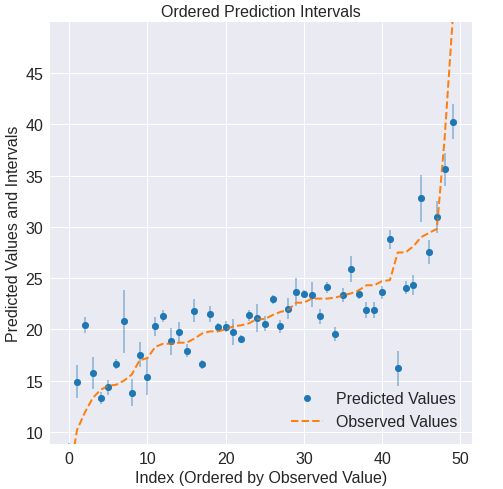
\includegraphics[width=\linewidth]{figures/eval/metrics/example_reg_metric_1.png}
         \caption{Underconfident predictions with $MPIW = 2.20$ and $PICP = 0.31$.}
     \end{subfigure}
     \hfill
     \begin{subfigure}[b]{0.49\textwidth}
         \centering
         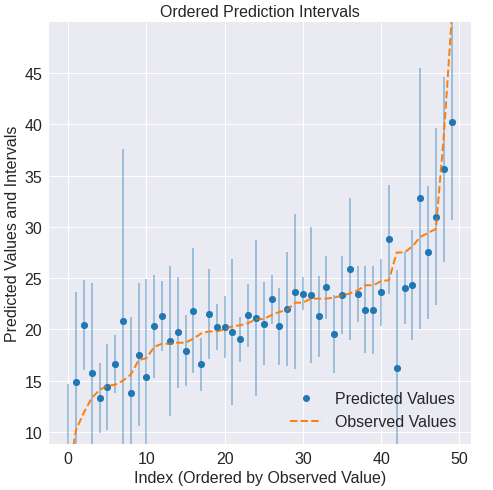
\includegraphics[width=\textwidth]{figures/eval/metrics/example_reg_metric_2.png}
         \caption{Calibrated predictions with $MPIW = 12.18$ and $PICP = 0.87$.}
     \end{subfigure}

        \caption{Example of the trade-off between the $MPIW$ and $PICP$ UQ metrics for regression.}
        \label{fig:example-uq-regression-metrics}
\end{figure}

\subsection{Classification}

Uncertainty quantification models for classification are usually evaluated using one of the following metrics:
\begin{itemize}
    \item Expected calibration error (ECE). It corresponds to the miscalibration area, i.e. the area between the reliability curve and the diagonal line in reliability plots. Given a set of exclusive data bins $\{B_l\}_l$ covering the calibration set $\bigcup_i B_l = X_{cal}$,  the ECE can be computed as follows. The lower the score, the better the calibration and, therefore, the quality of uncertainty quantification.
    $
    ECE = \sum_l \frac{|B_l|}{n} \mid acc(B_l) - conf(B_l)\mid
    $
    \item Brior score: another calibration metric, i.e. the equivalent of mean square error for predicted probabilities:
    $
    BS = \frac{1}{N} \sum_i {(p_{i,1} - y_i)^2} 
    $
    \item Oracle collaborative accuracy, f1 score, etc.\cite{collaborativeUQMetrics2021}. They measure the performance of the uncertainty quantification system under the capacity constraints of an oracle (e.g. human moderator). A given fraction of the testing dataset is forwarded to an oracle which returns the correct labels without errors. Only the most uncertain data points are selected to be labelled by the oracle: $D^{U}_\alpha = \{(x_i,y_i) \;:\: u_i = U(f, x_i) >= q_{1-\alpha} \}$ where $q_{1-\alpha}$ is the $1-\alpha$ quantile of the uncertainty scores series $\{u_i\}_i$. Given a scoring metric $M$, e.g. accuracy, the associated oracle collaborative metric $OC^M_{\alpha}$ is defined as
    $$
        OC^M_{\alpha} = (1 - \alpha) \cdot M(D \setminus D^U_\alpha) + \alpha 
    $$
    Intuitively, the better the uncertainty quantification, the more likely it is for $D^U_\alpha$ to contain prediction errors. The oracle collaborative accuracy is illustrated in figure \ref{fig:example-uq-classification-metrics}.
    \item Coverage checks for conformal predictions models\cite{conformalPredictions2021}: the equivalent of regression coverage metrics for classification, e.g. $\frac{1}{n} \sum_i I\{y_i \in C(x_i)\} \geq 1 - \alpha$
\end{itemize}


\begin{figure}
     \centering    
     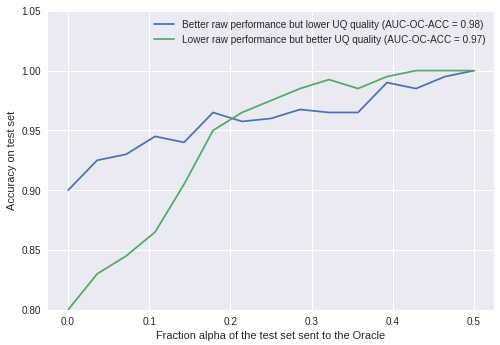
\includegraphics[width=0.67\textwidth]{figures/eval/metrics/oracle_collab_acc.png}
     \caption{Example of the evolution of the collaborative accuracy metric for two models as a function of $\alpha$. The \textit{green} model has a lower default accuracy but is better calibrated. At $\alpha=20\%$, it outperforms the \textit{blue} one.}
     \label{fig:example-uq-classification-metrics}
    
\end{figure}

The oracle-family of metrics is best suited for applications where humans are available for the labelling operation\cite{collaborativeUQMetrics2021}. However, in this work, it is used as a tool to assess the quality of uncertainty quantification models, which are uncoupled with the idea of oracle query ratio (or entropy threshold). To remove this dependence, we argue that the area under the oracle collaborative accuracy curve, i.e. $AUC-OC^{ACC}$,  is better suited to compare UQ models. Furthermore, this metric can be used during model selection to produce not only performing models but also calibrated ones. Indeed, if two models have a comparable accuracy score, the $AUC-OC^{ACC}$ metric favours the better-calibrated one.



\subsection{Factual uncertainty evaluation for graph-to-text} \label{factual-uq-metrics}

Classification UQ models are usually evaluated using metrics such as ECE or oracle collaborative accuracy. However, they are not particularly well-suited for text generation since multiple textual outputs are typically considered correct predictions. Furthermore, the oracle collaborative family of metrics are most relevant in an environment where the model can ask a human for help when it is uncertain about a prediction. In text generation, that is not very effective because humans have to intervene for each predicted token. For instance, a paragraph consisting of 50 words could require 5-10 manual checks, one per uncertain token, which is infeasible in practice, especially for many paragraphs.
Moreover,  LM calibration is often evaluated using downstream classification tasks (e.g. paraphrase detection), which is not relevant for the graph-to-text use case.
% factual point
Finally, none of these metrics can provide insights into the factuality of the model. Indeed, they are more focused on evaluating the uncertainty of the language model, which is less relevant to end-users than factual uncertainty. This also occurs with metrics such as BLEU, ROUGE or perplexity.

We propose to evaluate UQ models using factuality-aware metrics, i.e. reward models producing a high uncertainty score whenever a hallucination is generated. Given a hallucination entropy dataset $\Tilde{D} = \{(t_i, a_i, h_i)\}_{i=1}^N$ where $t_i \in V$ represent tokens, $a_i \in \{0,1\}$ hallucinations labels and $h_i$ the entropy for the token prediction $t_i$, we define the mean hallucination entropy (MHE) and the mean hallucination entropy difference $MHED$ as:

$$
MHE = \frac{ \sum_i a_i h_i }{\sum_i a_i}
$$

$$
MHED = \frac{\sum_i a_i h_i}{\sum_i a_i} -   \frac{ \sum_i \neg a_i h_i}{\sum_i \neg a_i}
$$


$\Tilde{D}$ can either be constructed synthetically via the procedure defined in section \ref{design:synthetic-hallucination-data} or via the hallucination detection models of section \ref{design:hallucination-detection-models}. These proposed metrics depend on the factuality of the model itself. In this work, it is evaluated using \textit{faithfulness}, which is defined as one minus the mean hallucination ratio\cite{factualityEnhancedLM} ($r_H$), i.e. the ratio between the number of hallucination entities to the total number of entities in the text:

$$
r_h(G,T) = \frac{ |HALLU_{NE}|}{|ALL_{NE(T)}|} = \frac{1 }{q}  \sum_{i=1}^q I\{NE(T)_i \not \in NE(G) \} \;\text{such that}\; q = |ALL_{NE(T)}|
$$
 Additionally, a variation of $r_H$, specialised on number-like tokens, is defined. It is referred to as the number hallucination or $r_h^{num}$. For the latter, $ALL_{NE(T)}$ is not computed using spaCy's default NER model but rather using the \textit{like\_num} property of tokens in spaCy (cf. \href{https://spacy.io/api/token}{documentation}).